\documentclass[notes,11pt, aspectratio=169]{beamer}

\usepackage{pgfpages}
% These slides also contain speaker notes. You can print just the slides,
% just the notes, or both, depending on the setting below. Comment out the want
% you want.
\setbeameroption{hide notes} % Only slide
%\setbeameroption{show only notes} % Only notes
%\setbeameroption{show notes on second screen=right} % Both

\usepackage{helvet}
\usepackage[default]{lato}
\usepackage{array}



\usepackage{tikz}
\usepackage{verbatim}
\setbeamertemplate{note page}{\pagecolor{yellow!5}\insertnote}
\usetikzlibrary{positioning}
\usetikzlibrary{snakes}
\usetikzlibrary{calc}
\usetikzlibrary{arrows}
\usetikzlibrary{decorations.markings}
\usetikzlibrary{shapes.misc}
\usetikzlibrary{matrix,shapes,arrows,fit,tikzmark}
\usepackage{amsmath}
\usepackage{mathpazo}
\usepackage{hyperref}
\usepackage{lipsum}
\usepackage{multimedia}
\usepackage{graphicx}
\usepackage{multirow}
\usepackage{graphicx}
\usepackage{dcolumn}
\usepackage{bbm}
\newcolumntype{d}[0]{D{.}{.}{5}}
\usepackage{subfigure}

\usepackage{changepage}
\usepackage{appendixnumberbeamer}
\newcommand{\beginbackup}{
   \newcounter{framenumbervorappendix}
   \setcounter{framenumbervorappendix}{\value{framenumber}}
   \setbeamertemplate{footline}
   {
     \leavevmode%
     \hline
     box{%
       \begin{beamercolorbox}[wd=\paperwidth,ht=2.25ex,dp=1ex,right]{footlinecolor}%
%         \insertframenumber  \hspace*{2ex} 
       \end{beamercolorbox}}%
     \vskip0pt%
   }
 }
\newcommand{\backupend}{
   \addtocounter{framenumbervorappendix}{-\value{framenumber}}
   \addtocounter{framenumber}{\value{framenumbervorappendix}} 
}

\setbeamertemplate{blocks}[rounded]
\setbeamercolor{block title}{bg=purple, fg=white}
\setbeamercolor{block body}{bg=purple!10}

\usepackage{graphicx}
\usepackage[space]{grffile}
\usepackage{booktabs}

% These are my colors -- there are many like them, but these ones are mine.
\definecolor{sage}{RGB}{102,153,102}
\definecolor{yellow}{RGB}{255,173,1}
\definecolor{purple}{RGB}{153,102,153}

% colors for diagrams
\definecolor{diagramtan}{RGB}{225,190,106}
\definecolor{diagramteal}{RGB}{64, 176, 166}
\definecolor{diagrampurple}{RGB}{170, 131, 239}
\definecolor{diagramred}{RGB}{146, 79, 79}


\hypersetup{
  colorlinks=false,
  linkbordercolor = {white},
  linkcolor = {sage}
}


%% I use a beige off white for my background
\definecolor{MyBackground}{RGB}{255,253,218}

%% Uncomment this if you want to change the background color to something else
%\setbeamercolor{background canvas}{bg=MyBackground}

%% Change the bg color to adjust your transition slide background color!
\newenvironment{transitionframe}{
  \setbeamercolor{background canvas}{bg=white}
  \begin{frame}}{
    \end{frame}
}

\setbeamercolor{frametitle}{fg=sage}
\setbeamercolor{title}{fg=sage}
\setbeamertemplate{footline}[frame number]
\setbeamertemplate{navigation symbols}{} 
\setbeamertemplate{itemize items}{$\rightarrow$}
\setbeamercolor{itemize item}{fg=sage}
\setbeamercolor{itemize subitem}{fg=sage}
\setbeamercolor{enumerate item}{fg=sage}
\setbeamercolor{enumerate subitem}{fg=sage}
\setbeamercolor{button}{bg=MyBackground,fg=purple,}



% If you like road maps, rather than having clutter at the top, have a roadmap show up at the end of each section 
% (and after your introduction)
% Uncomment this is if you want the roadmap!
\AtBeginSection[]
{
   \begin{frame}
       \frametitle{Roadmap of Talk}
       \tableofcontents[currentsection]
   \end{frame}
}
\setbeamercolor{section in toc}{fg=sage}
\setbeamercolor{subsection in toc}{fg=sage}
\setbeamersize{text margin left=1em,text margin right=1em} 

\newenvironment{wideitemize}{\itemize\addtolength{\itemsep}{10pt}}{\enditemize}

\usepackage{environ}
\NewEnviron{videoframe}[1]{
  \begin{frame}
    \vspace{-8pt}
    \begin{columns}[onlytextwidth, T] % align columns
      \begin{column}{.58\textwidth}
        \begin{minipage}[t][\textheight][t]
          {\dimexpr\textwidth}
          \vspace{8pt}
          \hspace{4pt} {\Large \sc \textcolor{blue}{#1}}
          \vspace{8pt}
          
          \BODY
        \end{minipage}
      \end{column}%
      \hfill%
      \begin{column}{.42\textwidth}
        \colorbox{green!20}{\begin{minipage}[t][1.2\textheight][t]
            {\dimexpr\textwidth}
            Face goes here
          \end{minipage}}
      \end{column}%
    \end{columns}
  \end{frame}
}

\title[]{\textcolor{sage}{Description of Hospital Leadership Data}}

\author[]{Hanna Glenn}
\date{\today}


\begin{document}

%%% TIKZ STUFF
\tikzset{   
        every picture/.style={remember picture,baseline},
        every node/.style={anchor=base,align=center,outer sep=1.5pt},
        every path/.style={thick},
        }
\newcommand\marktopleft[1]{%
    \tikz[overlay,remember picture] 
        \node (marker-#1-a) at (-.3em,.3em) {};%
}
\newcommand\markbottomright[2]{%
    \tikz[overlay,remember picture] 
        \node (marker-#1-b) at (0em,0em) {};%
}
\tikzstyle{every picture}+=[remember picture] 
\tikzstyle{mybox} =[draw=black, very thick, rectangle, inner sep=10pt, inner ysep=20pt]
\tikzstyle{fancytitle} =[draw=black,fill=red, text=white]
%%%% END TIKZ STUFF

% Title Slide
\begin{frame}
\maketitle
\end{frame}

\begin{frame}{end goal}
    \textcolor{purple}{the purpose of collecting this data is to get a sense of who is in charge of running nonprofit hospitals in the US}

    \vspace{10mm}

    why?
    \begin{wideitemize}
        \item we don't know a lot about who runs hospitals
        \item we know even less about whether characteristics of these people make a difference 
        \item for this project, I care specifically about the characteristic of clinical experience in executive positions
    \end{wideitemize}
\end{frame}


\section{Tax Form 990}

\subsection{who files?}

\begin{frame}{who files?}
\underline{important acronym:} EIN (Employer Identification Number)

    \centering
    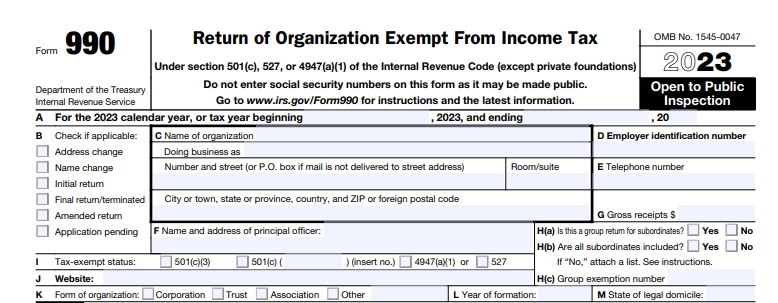
\includegraphics[scale=.7]{Graphics/990_snip_frontpage.PNG}
\end{frame}

\begin{frame}{who files?}
    \centering
    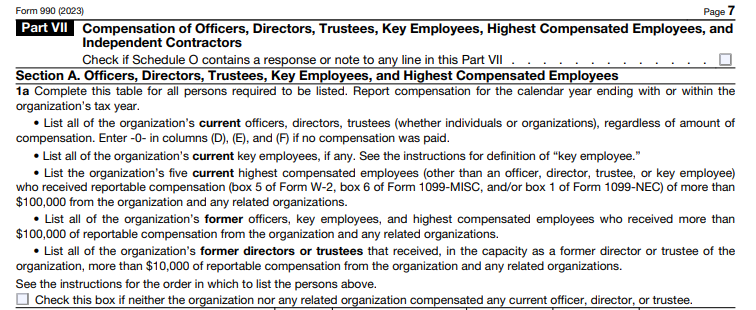
\includegraphics[scale=.7]{Graphics/990_snip_officerspage.PNG}
\end{frame}

\subsection{accessing hospital forms}

\begin{frame}{accessing hospital forms}\label{accessing hospital forms}
    \begin{wideitemize}
        \item completed forms are publicly available on ProPublica's website
        \item through their API, I download a list EINs classified as a hospital
        \begin{itemize}
            \item based on National Taxonomy of Exempt Entities (NTEE) codes: E20, E21, E22
        \end{itemize}
        \item along with EIN, I gather their name, zip, state, and urls to tax form pdfs
        \item years 2009-2015
    \end{wideitemize}

    \vspace{10mm}

    \begin{block}{data point}
        3,925 EINs \hspace{10pt} \hyperlink{why more?}{\beamergotobutton{why more?}}
    \end{block}
\end{frame}

\subsection{matching EIN to AHA hospitals}

\begin{frame}{matching EIN to AHA hospitals}
    I need to be able to link hospitals to other public data sets that capture hospital information
    \vspace{4mm}
    \begin{wideitemize}
        \item I choose to match to the widely used American Hospital Association survey data
        \item only match-able link I have is hospital name
        \item I restrict matches to being in the same state
    \end{wideitemize}
\end{frame}

\begin{frame}{matching EIN to AHA hospitals}
\centering
   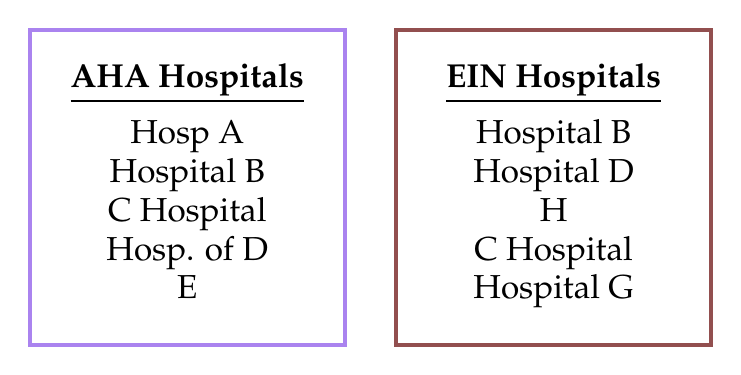
\begin{tikzpicture}[node distance=6mm, every node/.style={align=center, font=\large}]

        % Left box
        \node[draw=diagrampurple, line width=1.5pt, minimum width=4cm, minimum height=4cm, text=black] (ahaBox) at (0,0) {%
            \underline{\textbf{\textcolor{black}{AHA Hospitals}}} \\[4pt]
            \begin{tabular}{@{}c@{}}
                {Hosp A} \\
                {Hospital B} \\
                {C Hospital} \\
                {Hosp. of D} \\
                {E} \\
            \end{tabular}
        };

        % Right box
        \node[draw=diagramred, line width=1.5pt, minimum width=4cm, minimum height=4cm, text=black, right=of ahaBox] (einBox) {%
            \underline{\textbf{\textcolor{black}{EIN Hospitals}}} \\[4pt]
            \begin{tabular}{@{}c@{}}
                {Hospital B} \\
                {Hospital D} \\
                {H} \\
                {C Hospital} \\
                {Hospital G} \\
            \end{tabular}
        };

    \end{tikzpicture}
\end{frame}

\begin{frame}{matching EIN to AHA hospitals}
\centering
   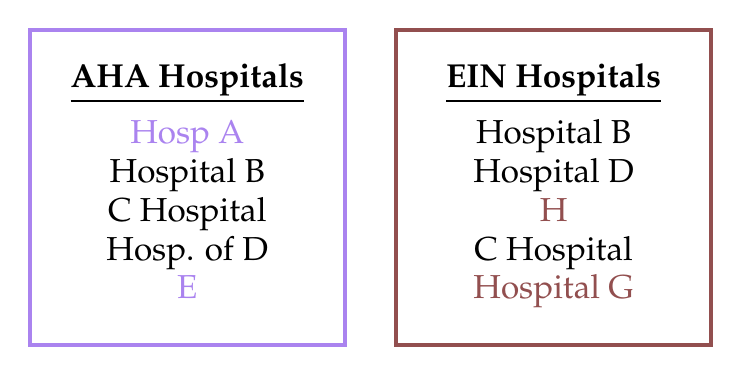
\begin{tikzpicture}[node distance=6mm, every node/.style={align=center, font=\large}]

        % Left box
        \node[draw=diagrampurple, line width=1.5pt, minimum width=4cm, minimum height=4cm, text=black] (ahaBox) at (0,0) {%
            \underline{\textbf{\textcolor{black}{AHA Hospitals}}} \\[4pt]
            \begin{tabular}{@{}c@{}}
                \textcolor{diagrampurple}{Hosp A} \\
                {Hospital B} \\
                {C Hospital} \\
                {Hosp. of D} \\
                \textcolor{diagrampurple}{E} \\
            \end{tabular}
        };

        % Right box
        \node[draw=diagramred, line width=1.5pt, minimum width=4cm, minimum height=4cm, text=black, right=of ahaBox] (einBox) {%
            \underline{\textbf{\textcolor{black}{EIN Hospitals}}} \\[4pt]
            \begin{tabular}{@{}c@{}}
                {Hospital B} \\
                {Hospital D} \\
                \textcolor{diagramred}{H} \\
                {C Hospital} \\
                \textcolor{diagramred}{Hospital G} \\
            \end{tabular}
        };

    \end{tikzpicture}
\end{frame}

\begin{frame}{matching EIN to AHA hospitals}
\centering
   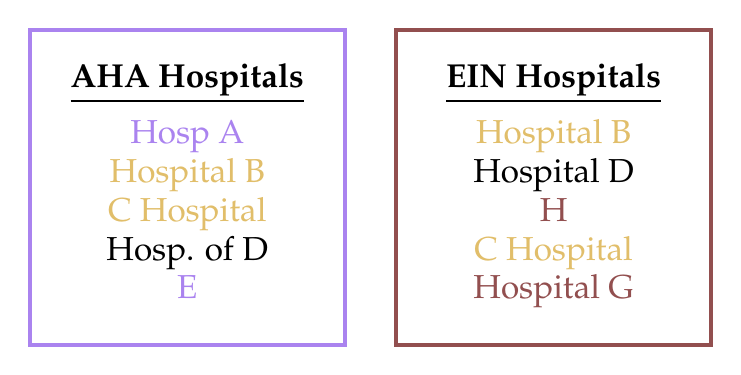
\begin{tikzpicture}[node distance=6mm, every node/.style={align=center, font=\large}]

        % Left box
        \node[draw=diagrampurple, line width=1.5pt, minimum width=4cm, minimum height=4cm, text=black] (ahaBox) at (0,0) {%
            \underline{\textbf{\textcolor{black}{AHA Hospitals}}} \\[4pt]
            \begin{tabular}{@{}c@{}}
                \textcolor{diagrampurple}{Hosp A} \\
                \textcolor{diagramtan}{Hospital B} \\
                \textcolor{diagramtan}{C Hospital} \\
                {Hosp. of D} \\
                \textcolor{diagrampurple}{E} \\
            \end{tabular}
        };

        % Right box
        \node[draw=diagramred, line width=1.5pt, minimum width=4cm, minimum height=4cm, text=black, right=of ahaBox] (einBox) {%
            \underline{\textbf{\textcolor{black}{EIN Hospitals}}} \\[4pt]
            \begin{tabular}{@{}c@{}}
                \textcolor{diagramtan}{Hospital B} \\
                {Hospital D} \\
                \textcolor{diagramred}{H} \\
                \textcolor{diagramtan}{C Hospital} \\
                \textcolor{diagramred}{Hospital G} \\
            \end{tabular}
        };

    \end{tikzpicture}

\vspace{7mm}
    
    \begin{block}{data point}
        I match 1,041 EINs to AHA hospitals using perfect name matching
    \end{block}
\end{frame}

\begin{frame}{matching EIN to AHA hospitals}
\centering
   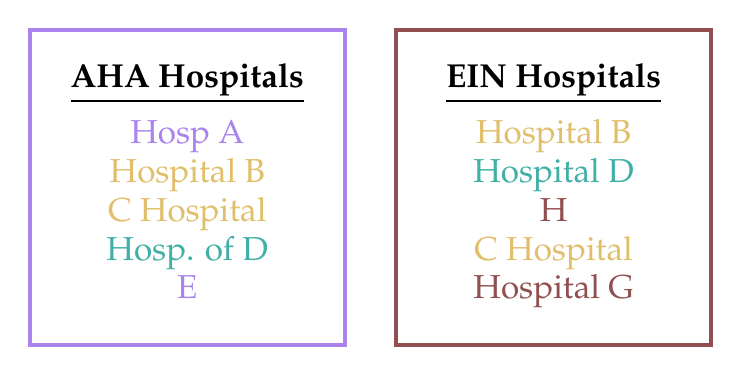
\begin{tikzpicture}[node distance=6mm, every node/.style={align=center, font=\large}]

        % Left box
        \node[draw=diagrampurple, line width=1.5pt, minimum width=4cm, minimum height=4cm, text=black] (ahaBox) at (0,0) {%
            \underline{\textbf{\textcolor{black}{AHA Hospitals}}} \\[4pt]
            \begin{tabular}{@{}c@{}}
                \textcolor{diagrampurple}{Hosp A} \\
                \textcolor{diagramtan}{Hospital B} \\
                \textcolor{diagramtan}{C Hospital} \\
                \textcolor{diagramteal}{Hosp. of D} \\
                \textcolor{diagrampurple}{E} \\
            \end{tabular}
        };

        % Right box
        \node[draw=diagramred, line width=1.5pt, minimum width=4cm, minimum height=4cm, text=black, right=of ahaBox] (einBox) {%
            \underline{\textbf{\textcolor{black}{EIN Hospitals}}} \\[4pt]
            \begin{tabular}{@{}c@{}}
                \textcolor{diagramtan}{Hospital B} \\
                \textcolor{diagramteal}{Hospital D} \\
                \textcolor{diagramred}{H} \\
                \textcolor{diagramtan}{C Hospital} \\
                \textcolor{diagramred}{Hospital G} \\
            \end{tabular}
        };

    \end{tikzpicture}

    \vspace{7mm}

    \begin{block}{data point}
        manually looking at names, I match 196 more EINs to AHA hospitals
    \end{block}
\end{frame}

\subsection{automated vs. manual collection}

\begin{frame}{automated vs. manual collection}
    I now have a list of EINs I want the pdfs for

    \vspace{4mm}

    \begin{wideitemize}
        \item I automate the download of the pdf URLs for these EINs that I collected from the API
        \item in many cases, the API misses the form even though it exists online
        \item I manually download the forms for which this error exists
    \end{wideitemize}
\end{frame}


\section{Text Extraction and Cleaning}

\subsection{optical character recognition}

\begin{frame}{optical character recognition}
    older pdfs are basically images, which requires using OCR for text recognition

    \vspace{4mm}

    \begin{wideitemize}
        \item the software takes pages and returns a string of text found
    \end{wideitemize}
\end{frame}

\begin{frame}{optical character recognition}
\begin{tikzpicture}
\node (bad) {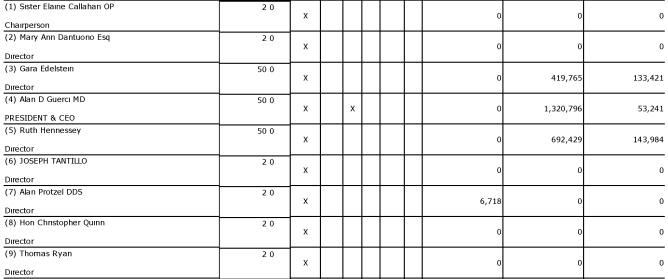
\includegraphics[scale=.5]{Graphics/990_snip_namesexample.PNG}};
\node (good) [right=of bad] {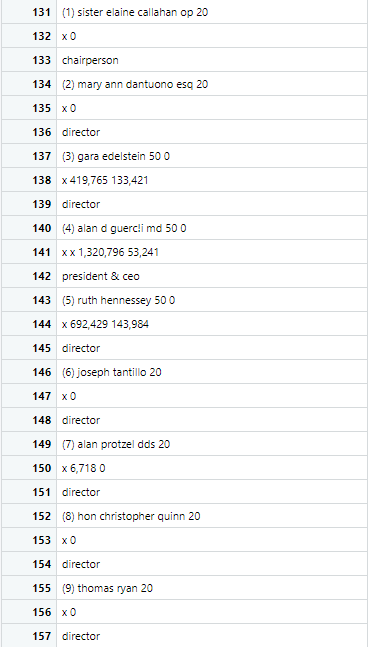
\includegraphics[scale=.45]{Graphics/r_snip_namesexample.PNG}};

\node (a) [fill=purple!50,draw] at (bad.center) {original pdf};
\node (b) [fill=purple!50,draw] at (good.center) {output from OCR};

\draw [ultra thick,purple,->] (a) to[bend left] (b);
\end{tikzpicture}
\end{frame}

\subsection{cleaning raw text output}

\begin{frame}{cleaning raw text output}
algorithmically locate names and associated positions

\vspace{4mm}

\begin{enumerate}
    \item remove numbers and special characters
    \item record full names where at least one (first or last) is found in census most common names data
    \item note when the name is followed by ``MD", ``DO", ``RN", etc. 
    \item locate the position nearest the name found and record it
\end{enumerate}
\end{frame}

\begin{frame}{cleaning raw text output}
    final names data:
    \vspace{4mm}
    \begin{wideitemize}
        \item each row is a name, hospital, year observation
        \item other variables: position, clinical experience
    \end{wideitemize}
\end{frame}



\section{Clinical Experience Characteristic}

\subsection{link names to NPPES}

\begin{frame}{link names to NPPES}
    next goal: verify and get more information on doctors in the data
    \vspace{4mm}
    \begin{wideitemize}
        \item use names to link to NPPES to get NPI number and specialty
        \item some cases are easy: MD in tax data and one name match to NPPES
        \item most are not that easy and require manual sleuthing
    \end{wideitemize}
\end{frame}




\begin{frame}{why more EINs than nonprofit hospitals?}\label{why more?}
    \begin{wideitemize}
        \item various sources quote the number of nonprofit hospitals to be less than 3,000
        \begin{wideitemize}
            \item (add citations)
        \end{wideitemize}
        \item without any limitations to hospital EINs at this point, my 3,925 EINs include hospital associations, fundraisers, and some large clinics that will later be excluded.
    \end{wideitemize}

    \vspace{10mm}

    \hyperlink{accessing hospital forms}{\beamerreturnbutton{go back}}
\end{frame}

\end{document}